%%%%%%%%%%%%%%%%%%%%%%%%%%%%%%%%%%%%%%%%%%%%%%%%%%%%%%%%%%%%%%%%%%% 
%                       rpithes-short.tex                         %
%         Template for a short thesis all in one file             %
%        (titlepage info below assumes masters degree}            %
%  Just run latex (or pdflatex) on this file to see how it looks  %
%      Be sure to run twice to get correct TOC and citations      %
%%%%%%%%%%%%%%%%%%%%%%%%%%%%%%%%%%%%%%%%%%%%%%%%%%%%%%%%%%%%%%%%%%% 
%
%  To produce the abstract title page followed by the abstract,
%  see the template file, "abstitle-mas.tex"
%
%%%%%%%%%%%%%%%%%%%%%%%%%%%%%%%%%%%%%%%%%%%%%%%%%%%%%%%%%%%%%%%%%%%

\documentclass{thesis}
\usepackage[english]{babel}
\usepackage[utf8x]{inputenc}
\usepackage{amsmath}
\usepackage{graphicx}   % if you want to include graphics files
\usepackage{algorithm}
\usepackage{algorithmicx}
\usepackage{algpseudocode}
\usepackage{url}
\usepackage[font=small,labelfont=bf]{caption}
\renewcommand{\algorithmicforall}{\textbf{for each}}
\let\ForEach\ForAll
% Use the first command below if you want captions over 1 line indented.
% A side effect of this is to remove the use of bold for captions. 
% To restore bold, also include the second line below.
%\usepackage[hang]{caption}     % to indent subsequent lines of captions
%\renewcommand{\captionfont}{\bfseries} % only needed with caption package;
                                        %   otherwise bold is default)
                                        
%%%%%%%%%%%%%%%%%%%%  supply titlepage info  %%%%%%%%%%%%%%%%%%%%%
\thesistitle{\bf Diffusive Load Balancing\\of Shape and Neighbor Counts}        
\author{Gerrett Diamond, Cameron Smith}        
\degree{Bachelors of Science}
\department{Mathematics} % provide your area of study here; e.g.,
%  "Mechanical Engineering", "Nuclear Engineering", "Physics", etc.
\thadviser{Mark Shephard}
%\cothadviser{First co-adviser} %if needed
%\cocothadviser{Second co-adviser} % if needed
%  For a masters project use \projadviser instead of \thadviser, 
%  and \coprojadviser and \cocoprojadviser if needed. 
\submitdate{March 2015\\(For Graduation May 2015)}        
%\copyrightyear{1685}  % if date omitted, current year is used. 
%%%%%%%%%%%%%%%%%%%%%   end titlepage info  %%%%%%%%%%%%%%%%%%%%%%
      
\begin{document} 
\titlepage             % Print titlepage   
\tableofcontents       % required 
%\listoftables          % required if there are tables
%\listoffigures         % required if there are figures

\specialhead{ABSTRACT}
Massively parallel mesh simulations require the mesh to be distributed
throughout many processes(parts) and be balanced in terms of computation and
communication. 
Many algorithms exist that target having an equal number mesh entities of a
specified dimension on each part. 
The most powerful of these, in terms of partition quality and run time are the
malt's-level (hyper)graph-based methods and the recursive geometric sectioning
methods. 
Multi-level (hyper)graph methods describe the mesh in terms of graph nodes and
(hyper)edges and then use a v-cycle of coarsening followed by un-coarsening to
divide the graph into subgraphs while recursive sectioning geometric methods use
a coordinate system such as the Cartesian location or centroids to recursively
section the mesh along coordinate or inertial axis. 
The faster geometric methods tend to create parts that have large inter-part
surface area, and many neighbors relative to the (hyper)graph based methods
which causes an increase in communication.
(Hyper)Graph-based methods can also suffer from similar issues as the number of
parts gets very large and the number of elements per part drops to several
hundreds. 
An alternative method that uses mesh data directly, ParMA, performs load 
balancing without the need to construct a graph. 
With access to all the mesh, partition, and model data, including topological 
and geometric coordinates, partitioning methods analogous to those used by 
(hyper)graph and geometric based procedures can be defined.
Towards this, ParMA partitioning methods will be extended to improve the 
overall shape of a part in order to reduce the number of neighbors each part 
has and thus reduce application communication times.

\newpage

\begingroup
\let\clearpage\relax

\chapter{INTRODUCTION}

%Descrube an unstructured mesh and its uses in the scientific world
In many scientific applications, mathematical models are used to develop 
simulations of real world scenarios. These models often are discretized over
either two dimensional or three dimensional unstructured mesh of vertices, 
edges, 
faces, and regions (for three dimensional meshes).  Complexities in the model 
and the domain can easily require meshes with billions of elements.
To run a simulation of this size it is necessary to distribute the elements 
across hundreds of thousands of processors where each processor gets a portion 
of the elements, a mesh 'part'.

To ensure the effectiveness of distributing the mesh among parts it is 
important to balance the loads evenly throughout the parts. This load is 
expressed as the combination of the computational costs and the communication 
costs which depend on the application. Computational costs include the 
application's work that has to be done on the local elements of the part. The 
communication costs involve sending and receiving information between parts, 
often defined by mesh entity adjacencies across part boundaries. Balancing 
both of these based on the application leads to the least overhead of the 
application.
%This doesn't flow very well anymore but it is salvagable I think

When communication costs are measured by, or a direct result of, the number 
of entities cut by part boundaries the costs can be lowered by (1) reducing 
the number of entities cut by the boundary and (2) reducing the number of 
parts, processes, a part borders.  The former objective is the typical 
secondary objective of most partitioning tools, reducing the cut size.  The 
latter objective, assuming equal cut size, reflects the potentially increased 
cost of sending several small messages to many endpoints versus sending large 
messages to fewer endpoints \cite{MPIpresent,MPImessage}.

Typical parallel mesh load balancing algorithms target distributing the 
computational load of an application evenly across all parts. Even with the 
computational load of each part balanced, a part with many neighbors can have 
increased communication overheads. In order to fix such boundary problems a 
balancing algorithm must take into account the overall shape of the parts. 
More precisely the algorithm must try to remove part boundaries cutting only a 
small number of mesh vertices.

The work presented here suggests a method that given a mesh will 
increase the length of small part boundaries. Our work 
sends a small number of elements bounded by the ends, in 2D the endpoints of 
the line formed by the part boundary, in 3D the segments bounding the part 
boundary surface, of the targeted part boundary to incrementally increase its 
size. The format of the paper is as follows. Section 2 
discusses common approaches to mesh load balancing and there use in shape 
correction. Section 3 describes our algorithm to fix part shape. Section 4 
shows results from our testing. Section 5 and 6 list our plans to improve the 
method. Some terminology used in the paper is defined as follows:

{\bf Mesh Entity } - A piece of the mesh representation of order $d$ where $d \in [0,3]$ which refers to vertex, edge, face, region in order.

{\bf Element} - A mesh entity that is a face for a two dimensional mesh or a region for a three dimensional mesh.

{\bf Imbalance of order $d$} - the maximum number of entities of order $d$ on any part divided by the average across all parts

{\bf Boundary length} - the number of vertices along a boundary of two parts.

{\bf Small Side/Boundary} - a boundary between two parts that has a boundary length less than a given percentage of the average boundary length.


\chapter{Related Works}
Many different distributed methods to balance unstructured meshes have been 
explored in the past \cite{multidiffuse,surveygraph}. Here we discuss the 
three most commonly used methods: graph/hypergraph, diffusive, and multilevel.

\section{(Hyper)graph methods}
Graph and Hypergraph load balancing methods use an abstraction of the mesh in 
order to balance the work load between processes. The first step to using 
hypergraph/graph methods is creating this abstraction. Zhou et al. define that 
the graph nodes are built off of a specific mesh entity typically either faces 
for 2D or regions for 3D \cite{zhougraph}. The edges are then built based on the
dependencies of the nodes. In their work they found that using only a subset of 
these edges is sufficient for the same quality of partition. For their work with
regions as nodes they found using the face adjancencies gave just as good a 
partition in much less time. The authors also define two different types of 
edges: Interedges that connect graph nodes on different processors and 
intraedges that connect graph nodes on the same processor. Zhou describes the 
hypergraph as an extension of the graph where hypergraph nodes are the same as 
graph nodes, but hypergraph edges or hyperedges represent dependencies between 
more than one mesh entity. Thus hyperedges can correlate each entity with all 
of its face adjancencies. The overall goal of hypergraphs and hyperedges is to 
partition the graph while minimizing the number of parts the hyperedges extend 
over.

Buluc et al. \cite{surveygraph} give an overview of graph methods in the field 
for both graphs and hypergraphs. They also discuss the challenges and 
NP-hardness of many of the algorithms for graph balancing. Two metrics that 
are used to model the overall shape for graph methods are the edge cut and 
communication volume. The authors show that communication volume is a better 
measurement which leads to hypergraph methods which better target the 
communication volume because hyperedges represent the number of different 
neighboring parts to each node in the graph. Devine et al. discuss methods 
to use hypergraphs for parallel scientific computing \cite{hypergraph}. They
use hypergraphs to accurately represent communication volume and as a result
part neighbors. The hypergraph method uses hyperedges or nets which connects 
several nodes in the graph that may be on different parts. Therefore 
balancing a hypergraph naturally puts an effort towards balancing the overall
shape and neighbors of parts. 

Graph and Hypergraph methods for load balancing are said to be the most 
effective \cite{zhougraph,surveygraph}. Still there are some draw backs 
presented by Zhou et al. \cite{zhougraph}. First off since the graph targets 
a specific dimension, the other dimensions can become unbalanced. Also 
graph/hypergraph methods do not scale well when working with more than 
100,000 processors. The authors explain that using both local partitioning 
and global partitioning can result in good partitions that can scale out to
large part counts. Also with large part counts some parts become much 
heavier than others which limits the scalability of these methods.

\section{Diffusive load balancing}
Willebeek-LeMair and Reeves describe diffusive load balancing techniques with 
four steps \cite{loadbalance}. The first is evaluating the processor load, then 
determining the profitability of the load balancing, followed by a task 
migration strategy, and finally a task selection strategy. They review over 
five different strategies and how they perform on the second and third task. 
The first method reviewed was the Sender Initiated Diffusion method (SID). 
This method restricts parts to only communicate with their neighbors and the 
heavy parts or senders are the migration selectors. The second technique is 
similar to the first and called Receiver Initiated Diffusion (RID). Once again 
parts can only communicate with their neighbors, but instead of the heavy parts
selecting migration targets, the light parts select heavier neighbors to receive
load from. Our method for shape optimization is similar to the idea of a RID 
method. In the Gradient Method (GM), light parts inform nearby parts in search 
of a heavy part which causes heavy parts to send load towards the closest light 
part. The Hierarchical Balancing Method (HBM) breaks up load balancing into a 
hierarchy of parts and performs load balancing at a low level and then continues
to balance while moving up a hierarchy. The final method is the Dimension 
Exchange Method (DEM). Similar to the HBM, the DEM approach balances at a low 
level and works up, but the DEM balances synchronously in all dimensions one at 
a time.

Zhou et al. developed a diffusive algorithm to balance the heavy parts produced 
by graph/hypergraph methods \cite{zhougraph}. They target balancing the mesh vertices for each
part of the partition by offloading certain entities from heavy parts to 
lighter parts. Their method, the local iterative interpart boundary 
modification algorithm (LIIPBMod), identifies mesh vertices on the heavy parts
that are bounded by a small number of elements. By doing this, LIIPBMod 
balances the vertex partitioning while still maintaining the element balance
produced from the graph/hypergraph partition. This process when repeated 
results in a partition that has vertex balance with a minor decrease in the 
good element balance. The results of their method shows a dramatic improvement
of vertex imbalance sometimes reducing from over 20\% to around 5\%. They 
discuss that the scaling is not so significant because much more time is spent 
on the graph/hypergraph partitioning than their method.


\section{Multilevel methods}
Buluc et al. describe the multilevel methods as the most successful approach to 
graph partitioning \cite{surveygraph}. They describe multilevel methods 
generally as a three step process. The first step is to coarsen the mesh 
until some threshold in order to reduce complexity. The second is to create 
an initial partition of this fully coarsened mesh that can be done much 
faster than the entire mesh. Next the mesh is refined in the opposite direction
of the coarsening. At each step the mesh is progressively refined in order to
keep the balance across the parts. This design is called a v-cycle. The 
generality of the design allows most algorithms to be altered to work in a 
multilevel form. 

Meyerhenke et al. port a diffusive method previously used for 
shape optimization into a multilevel algorithm \cite{multidiffuse}. They use a 
previously used distributed load balancing algorithm, Bubble-FOS/C (First order
diffusion scheme with constant drain) for load balancing in their multilevel
method. This Bubble method is an iterative scheme based on Lloyd's k-means 
algorithm. This method involves solving linear systems repeatedly which causes 
a high run time. Thus the authors introduce a second balancing algorithm, 
TruncCons (truncated diffusion consolidations), into the v-cycle. This 
algorithm is faster than Bubble for large mesh sizes and is used for small
diffusive improvements. They use the multilevel structure in order to use 
the expensive but more effective Bubble-FOS/C when at the small levels of the 
v-cycle and then use TruncCons to balance the larger parts of the v-cycle. 
This method was shown to be much faster than the original method 
of just the Bubble-FOS/C and also produces a better quality of load balancing. 
They compared this new method to the popular methods KMetis and JOSTLE and 
found their method to produce higher quality partitions but still having a
much higher run time. They expect reasonable scaling for the algorithm but 
results show the algorithm taking minutes rather than seconds like other 
methods.

\chapter{Method}

The approach we take to fixing small sides builds off a parallel 
dynamic partitioning framework called ParMA \cite{parma}. Thus our algorithm, Gap,
 defines a series of steps defined in the ParMA load balancing method to target
 small sides and migrate elements to increase the size of these boundaries. Here 
we describe the base framework of ParMA and how it is extended to create Gap.

\section{ParMA}

ParMA load balancing methods follow a five step plan. These five steps 
are the sides determination, weight assignment, target phase, selection
phase, and the stepper phase. The sides determination is when each part 
determines which parts are its neighbors. These sides are defined for some
 dimension $d$ as a part that shares a mesh entityof order $d$. After sides are 
determined, the weight assignment phase collects the weight (for a certain 
mesh entity order (vertex, edge, face, or region)) of the neighbor parts 
defined by the sides. The 
target phase defines which parts will be sending and the parts each one 
will be sending to. The target phase also defines an amount of weight to 
be transferred from each sending part to each of its targets. The selection 
phase determines which elements of the mesh will be sent to the targets 
until the given amount of weight is satisfied. The final stepper phase is 
to migrate the elements between each part and complete the load balancing 
step. These steps are repeated until a stopping criteria is satisfied 
during the stepper phase. 

Each diffusive load balancing algorithm derived from ParMA implements these 
steps to target the criteria of the algorithm \cite{parma}. The most important 
steps of the ParMA framework is the target phase and selection phase which 
defines the problem specific actions that will be taken to balance the parts. 
The stopping criteria is typically to go below some balancing threshold of 
a given mesh entity order(s). We define the balancing threshold to be a 
percent imbalance of the given mesh entity order among all of the parts. 
The percent is typically between 1\% and 10\%. The stopping criteria can also 
be appended to include problem specific endpoints.
 
  
\section{Gap}

Gap derives from ParMA and thus must define the phases to sepcifically target 
small boundaries and select elements around the small boundaries in order 
to increase the length of these small sides. 

\subsection{Vertex Sides}

For sides, we decide to use vertex sides ($d$=0) in order to represent the 
boundaries between two parts. We choose this in order to locate single vertex 
junctions between parts. Fixing these single vertex junctions allows gap to 
decrease the number of neighbors by turning the single vertex junction into 
a small side that can later be increased. The sides are also used to count how 
many vertices a given boundary has. This quantifies the length of the 
boundaries for the later phases of the algorithm.

\subsection{Receiver based targeting}

%General Discussion
Gap uses a reverse method of deciding targets. The targets of Gap are the 
parts that share a small boundary. To detect these small boundaries the 
targets must detect themselves rather than the senders. Thus, Gap 
implements a receiver based targeting where parts detect that they are 
receivers and inform the sending parts to send elements to the receivers. 

%Description of Algorithm
Algorithm \ref{alg:targets} outlines the method for finding small sides 
and determining the sending parts. First each part finds the smallest 
boundary it has and checks if the length of this boundary is less than 
a given percentage of the average length of all boundaries. Each iteration 
the percentage that is multiplied by the average side length increases 
towards 100\%. Once the small sides are found, pairs of parts that share 
these small boundaries attempt to confirm each other. All of the matches 
that are found become the receivers of this step. The receivers then 
traverse along the small boundary to find the parts that share a vertex 
with the two receiving parts. Figure \ref{fig:boundary} shows an example 
of this. Parts one and two detect the small boundary which then determine 
parts zero and three as the senders. The receivers then send messages to the 
senders to inform them. At that point the senders set each receiver as a 
target and calculates the number of elements to send to the targets 
based on the difference between the average length of a side and the 
small side's length.

\begin{figure} [!h]
\centering
\captionsetup{justification=centering,margin=1cm}
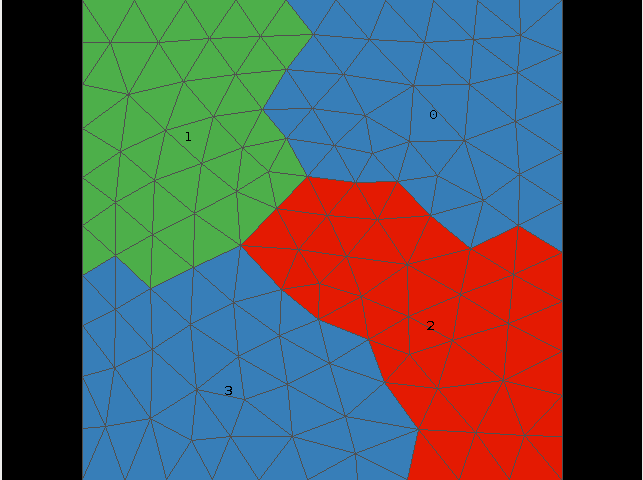
\includegraphics[width=.6\textwidth]{target_example.png}
\caption{\label{fig:boundary} \textnormal{Four part plate mesh after targeting phase. Part two(red) finds the small side with part one(green). Part one labels the parts zero and three (blue) as the senders.}}
\end{figure}

\begin{algorithm}
\caption{Gap Target phase}
\label{alg:targets}
\begin{algorithmic}[1]
\Require {mesh $M$ of dimension $d$, sides $s$, weights $w$}
\Procedure{targets}{$M$, $s$, $w$}
  \State $targets \leftarrow \emptyset$
  \If {part is in MIS subset AND smallest\_side$<$tolerance}
    \State $other = $ part opposite small side
    \State send message to $other$
  \EndIf
  \If {receives message}
    \State $other = $ message sender
    \State $senders \leftarrow findNeighbors() - self - other$
  \EndIf
  \ForEach {$send \in senders$}
    \State send self and other in message to send
  \EndFor
  \If {receives message}
    \State $targets \leftarrow [parts,calcWeight(parts)]$
    \State $targets \leftarrow [secondpart,calcWeight(second)]$
  \EndIf
\EndProcedure
\end{algorithmic}
\end{algorithm}


\begin{figure} [hb]
\centering
\captionsetup{justification=centering,margin=1cm}
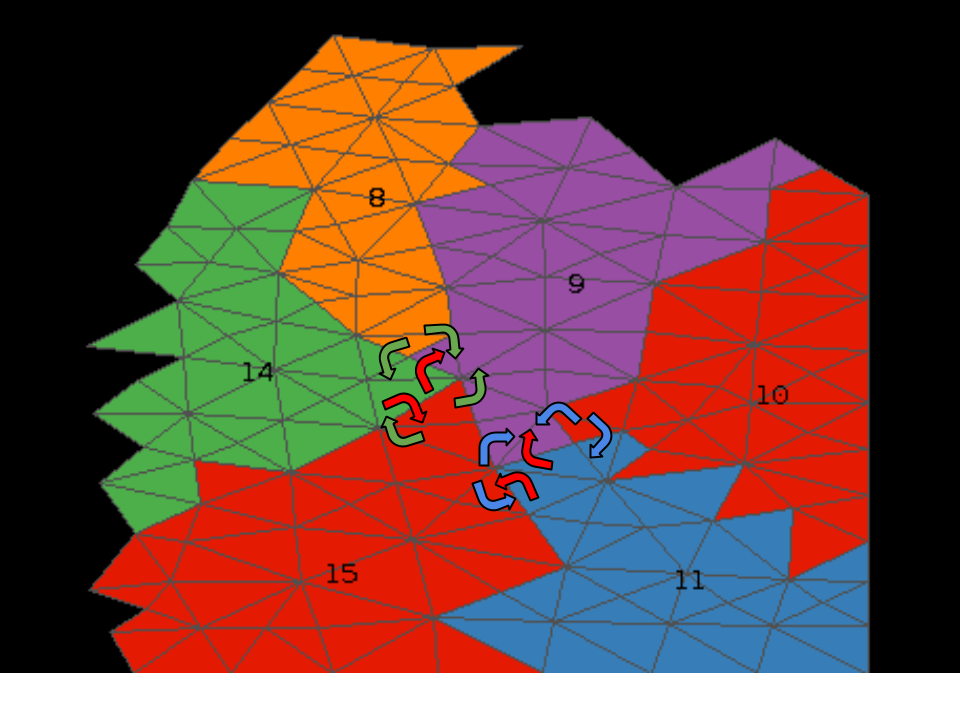
\includegraphics[width=.6\textwidth]{MIS_problem.png}
\caption{\label{fig:recvsend} \textnormal{Possible error if two small sides occur next to each other. There are small boundaries between parts nine and eleven, nice and fourteen, and nine and fifteen. Arrows show migration direction for the color of the part finding the small side. Conflicts exist between the migrations of the fifteen-fourteen boundary and the fifteen-eleven boundary}}
%REALLY long caption...
\end{figure}

% Maximal Independent Set
One problem that can occur during the target phase is if a part is 
designated as a receiver and a sender. This causes elements to be sent 
to the part and from the part in the same migration which will cause 
disconnected components throughout the boundary between the parts. In Figure 
\ref{fig:recvsend} Gap finds small sides on the boundaries eleven-nine, 
fouteen-nine, and fifteen-nine.
The arrows in the figure shows the resulting direction of migration. The color 
of an arrow represents the migration caused by the small side of that color. 
For example the red arrows are for the fifteen-nine boundary migration. There 
are 
conflicts that occur in the migration along the fourteen-fifteen boundary and 
the eleven-fifteen 
boundary where elements are migrated in both directions.  Our solution to this 
problem is to not allow neighboring parts to send to each other by using a 
maximal independent sets (MIS) of non-neighboring parts. We used Luby's 
randomized parallel MIS algorithm \cite{luby} to separate which parts find the 
small boundaries by making subsets of the parts such that none of the parts 
within a subset are neighbors to each other. Thus each step of the load 
balancing algorithm uses a different subset from the maximal independent sets. 
So the first part of the target phase is each part in the MIS subset 
finds its smallest side. If this side is less than the percent of the average 
side length then it sends a message to the part on the other side of the 
boundary. This other part then determines the senders and the rest of the 
algorithm follows. These changes to the target phase are included in Algorithm 
\ref{alg:targets}. The MIS subsets guarantee that two adjacent parts cannot 
find small sides that would cause the sender and receiver conflict. 
%do I add reference to the above figure too???



\subsection{Selection by Centroid}
After targets have been found each sender must choose which elements close 
to the small side will be migrated to the neighboring parts and which part 
each element will migrate to. To do this Gap's selection phase uses geometric 
centroids to determine which elements to send first and which part will 
receive them. The process begins with the sender part determining a seed 
element that is vertex adjacent to the small side. As there is likely 
multiple elements adjacent to the small side boundary we use the element 
that is furthest from the centroid of the part. This is found by the euclidean 
distance from the element's centroid to the part's centroid. Once the seed 
element is selected additional elements are chosen that 
are adjacent by one mesh entity order less than the dimension of the mesh 
(edge in two dimensions and face in three dimensions). Each additional edge 
is added to a priority queue that is sorted by the distance of the element 
to the part centroid. This queue is traversed continuously adding more 
elements until the sum of the elements weight sent is greater than the total 
weight calculated in the targets phase. This selection causes the sender 
parts to become rounder as the furthest away elements are sent first.

Since each sender has two target parts, one on each side of the small 
boundary, each element to be migrated must choose one of the target parts to 
migrate to. We choose to send each element to the closest part geometrically. 
The closeness of an element to a part is defined as the euclidean distance 
from the elements centroid to the target part's centroid. Thus the element 
is migrated to the receiving part that has the lower of these distances. 
These migration choices lead to the small side being extended towards the 
sender parts. 
%A simple example is shown in Figure \ref{fig:selection}. Here 
%the small side is between parts \# and \#. The black represents the initial 
%boundary lines and the red is the boundaries after a step of the shape 
%balancing.


\subsection{Stopping Criteria}
% reorder discussion of this at some point.
Gap's goal is to increase the length of small boundaries
Gap does not directly attempt to decrease the imbalance of entities within 
the mesh. In fact, Gap will sacrifice imbalance in order to achieve an improved 
shape quality. Therefore the stopping criteria for Gap is when it goes above a 
given level of imbalance. In addition to the imbalance criteria Gap also 
finishes once the minimum boundary length is greater than a percentage of the 
original average boundary length. With both of these conditions Gap will 
complete if the mesh becomes too imbalanced or the smallest sides have been 
widened towards the average. For our tests we used 20\% imbalance and 70\% 
of the initial average side length. We choose 20\% imbalance because this 
imbalance is still easily fixed by ParMA entity imbalance improvement 
\cite{parma,zhougraph,zhou2012}.

\chapter{Results}

Our initial testing of Gap has been done on a two dimensional flat plate mesh. 
A 16 part version of the plate mesh partitioned by  the Recursive Inertial 
Bisection (RIB) method \cite{williamsRIB,taylorRIB} is included in Figure 
\ref{fig:plate}. There are single vertex junctions between parts 
zero-one-two-three, 
parts four-five-six-seven, parts one-five-seven-eight, parts 
seven-eight-twelve-forteen, and parts one-three-eight-nine. There are 
also two vertex sides on the thirteen-fourteen boundary, the nine-fifteen 
boundary, and seven-twelve 
boundary. Gap was run on the mesh until the smallest boundary was three after 
nine 
iterations of the balancing algorithm. Figure \ref{fig:plate_gap} shows the 
resulting mesh. Here all of the single vertex junctions have been replaced with 
new part boundaries and increased accordingly. Also several boundaries were 
altered to even out the lengths to at least three. Several larger cases of gap are run and shown in Figures \ref{fig:gap1}, \ref{fig:gap2}, and \ref{fig:gap3}. These are larger 16 part plate meshes with 876 faces, 1273 faces, and 1885 faces respectively.  \\[5cm]

\begin{figure} [!hp]
\centering
\captionsetup{justification=centering,margin=1cm}
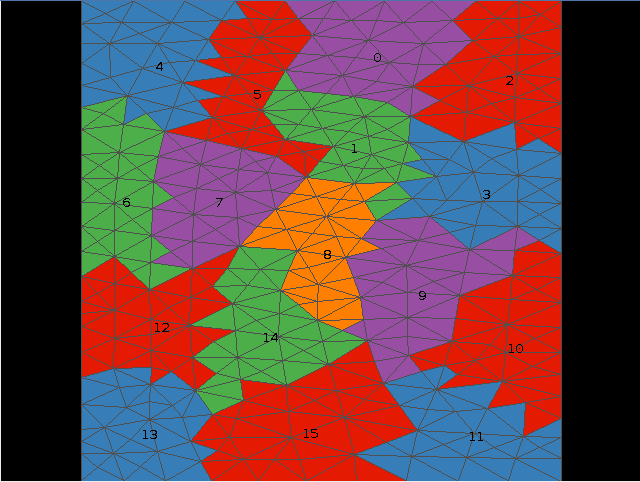
\includegraphics[width=.6\textwidth]{results_before.png}
\caption{\label{fig:plate} \textnormal{16 part plate mesh with 634 faces before Gap is run. Small sides exist between parts thirteen and fourteen, nine and fifteen, etc. Several single vertex junction exist like the one between parts zero, one, two, and three}}
\end{figure}

\begin{figure} [!hp]
\centering
\captionsetup{justification=centering,margin=1cm}
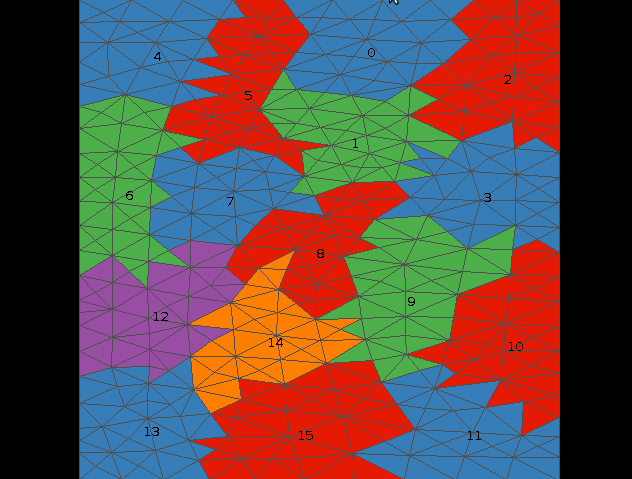
\includegraphics[width=.6\textwidth]{results_after.png}
\caption{\label{fig:plate_gap} \textnormal{The same 16 part plate mesh after Gap has been run. The single vertex junctions have been removed and the minimum side length has been increased to three.}}
\end{figure}


\begin{figure} [!h]
\centering
\captionsetup{justification=centering,margin=1cm}
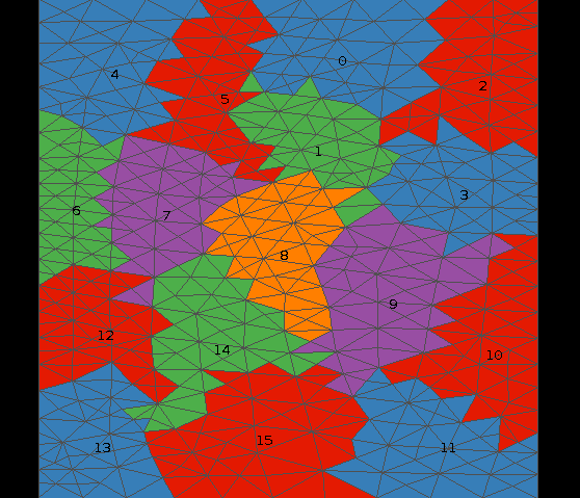
\includegraphics[width=.4\textwidth]{before_876.png}
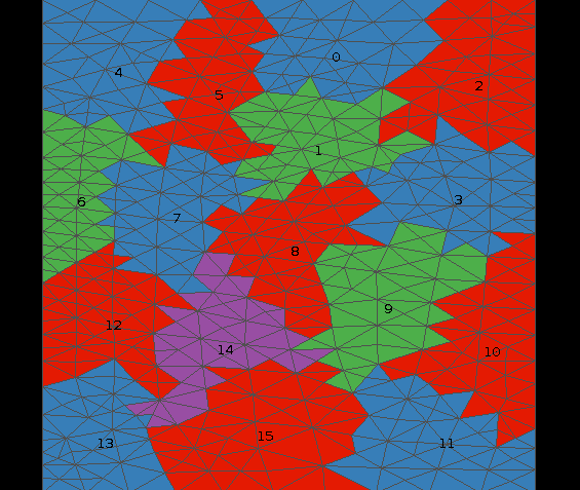
\includegraphics[width=.4\textwidth]{after_876.png}
\caption{\label{fig:gap1} \textnormal{16 part plate mesh with 876 faces before gap (left) and after gap (right)}}
\end{figure}

\begin{figure} [!h]
\centering
\captionsetup{justification=centering,margin=1cm}
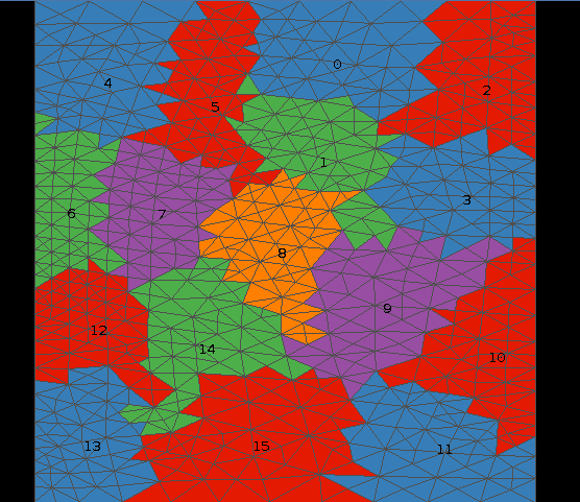
\includegraphics[width=.4\textwidth]{before_1273.png}
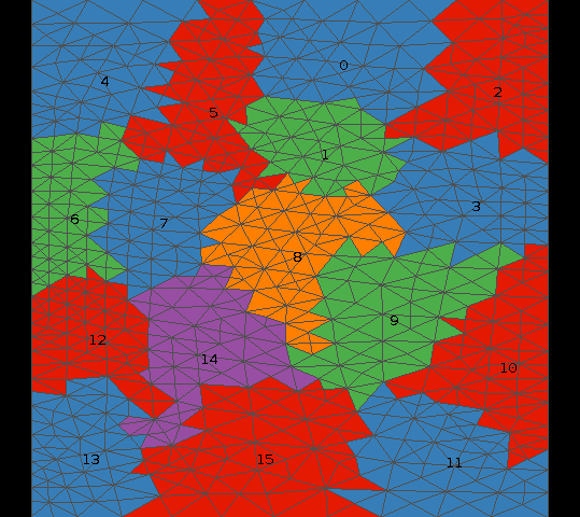
\includegraphics[width=.4\textwidth]{after_1273.png}
\caption{\label{fig:gap2} \textnormal{16 part plate mesh with 1273 faces before gap (left) and after gap (right)}}
\end{figure}

\begin{figure} [!h]
\centering
\captionsetup{justification=centering,margin=1cm}
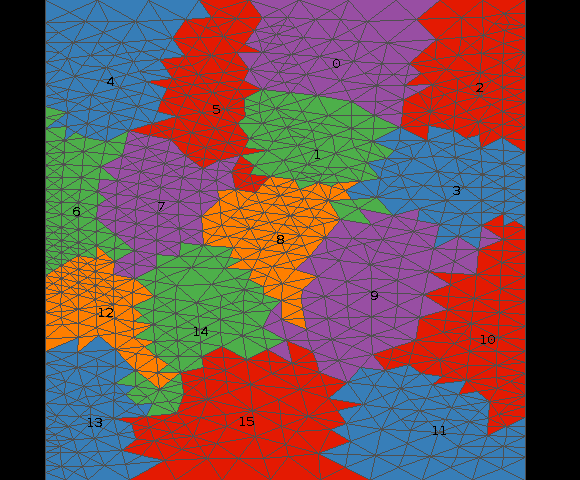
\includegraphics[width=.4\textwidth]{before_1885.png}
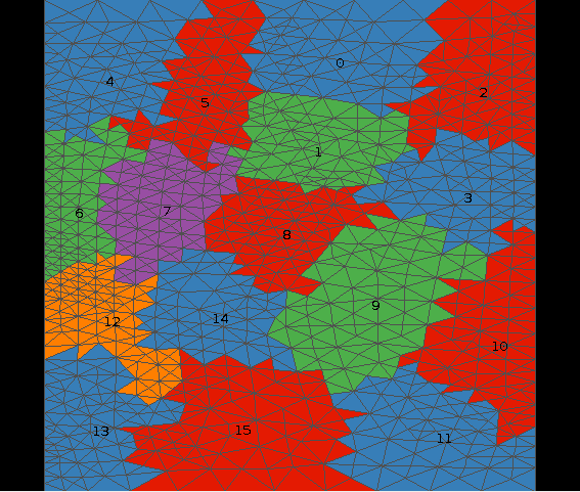
\includegraphics[width=.4\textwidth]{after_1885.png}
\caption{\label{fig:gap3} \textnormal{16 part plate mesh with 1885 faces before gap (left) and after gap (right)}}
\end{figure}


\chapter{Limitations and Future Work} 

%Testing (if not sufficient) 
%Make sure to move the first sentence of the next paragraph if added

%Geometric centroids to topological centroids
Gap is a work in progress and as such has several extensions required to make 
it a more general algorithm. First of all as seen in the Figure \ref{fig:gap3} 
after being balanced by gap, the boundaries are jagged and branch out in a 
nonuniform path which allows longer boundary lengths but a smoother boundary 
and more elliptical shape would be ideal.  These jagged boundaries are a 
result of using geometric centroids to compute distances for migration 
selection. The geometric centroid takes no topological information into account 
which causes the topology to be sacrificed in order to achieve the goal. In 
future testing we would like to try using topological centroids instead of 
geometric centroids. Topological centroids are defined by the distance from the 
boundary by a breadth first search traversal. This gives each vertex a number 
of the shortest path to the boundary. The topological centroid is the vertex 
with the highest number is defined as the topological centroid. Since this 
centroid is defined based on the actual boundary, the distance from the 
centroid is based on element distance rather than element size which leads to 
better topological choices.

%Small Isolated Components and non fixable regions
Due to the nature of Gap's targeting, there are some regions that cannot be 
fixed by Gap. Namely these are areas where there are no sender parts around 
the boundary between two parts. Currently if one of these regions is the 
smallest side between the two parts, the parts will continuously try to fix 
those small sides rather than target ones that have sender parts incident on 
the small side. We would like to have Gap ignore these un-fixable boundaries 
in order to target small sides that can be fixed by the algorithm. In Figure 
\ref{fig:ocean} there are several small red isolated components of the red 
part that cause a small side with the orange part. These sides cannot be 
increased because there are no parts next to the boundary to migrate elements 
to the red or orange parts.

\begin{figure} [!ht]
\centering
\captionsetup{justification=centering,margin=1cm}
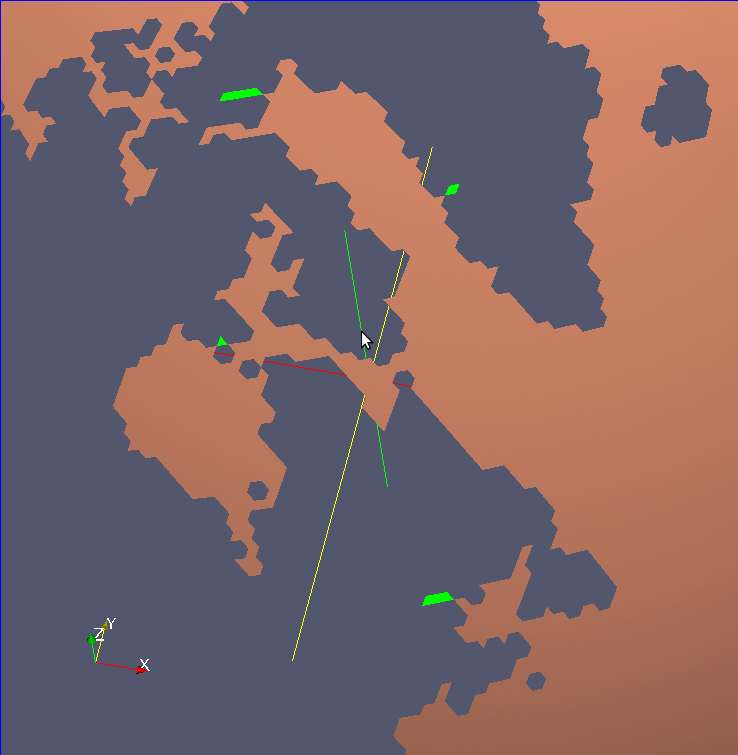
\includegraphics[width=.65\textwidth]{Ocean_Isolated.png}
\caption{\label{fig:ocean} \textnormal{Several isolated components that cause the two parts to have small sides that cannot be fixed by Gap since there are no parts next to the boundary.}}
\end{figure}


\chapter{Closing Remarks}

We presented a method to improve the shape of a mesh in order to reduce 
communication costs across different processes. Out implementation worked off of 
a parallel dynamic partitioning framework, ParMA, to target small boundaries 
and migrate elements at the end of the boundaries based on distances from 
centroids to increase the length sides. The key to our method is improving 
shape at the cost of small imbalance increases which can be quickly recovered 
with ParMA diffusive improvement procedures without losing the shape 
improvements. Our initial testing shows for a simple two dimensional mesh that 
Gap successfully lengthens the small edges and removes single vertex junctions. 
Since the plate mesh is 
simplistic there were several extra considerations that must be implemented 
to create a method that works in general cases of both two dimensional and 
three dimensional meshes. 

\endgroup

% The following produces a numbered bibliography where the numbers
% correspond to the \cite commands in the text.
\specialhead{LITERATURE CITED}

%\newpage
\bibliographystyle{plain}
\bibliography{references.bib}

\end{document}
